%author : Hanna Svennevik
\begin{figure}[hp]
    \centering
    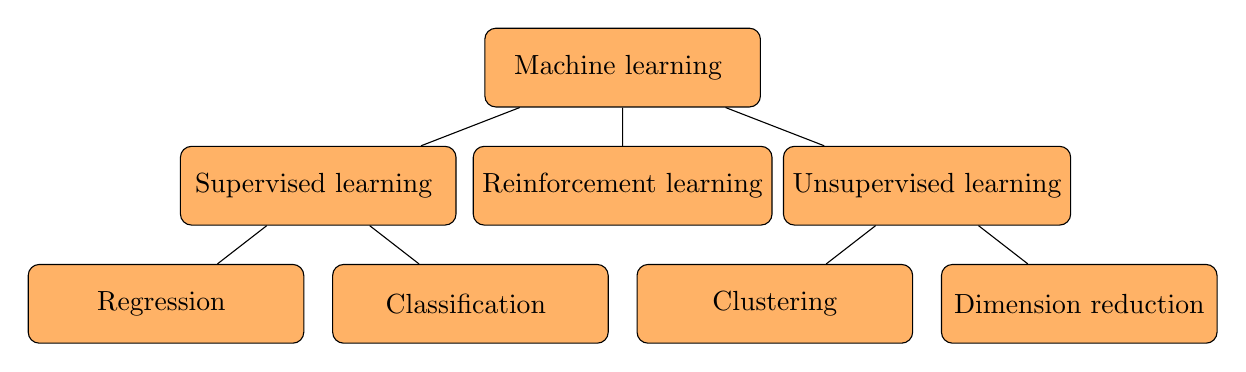
\begin{tikzpicture}[sibling distance=11em,
  every node/.style = {shape=rectangle, rounded corners,
    draw, align=center, 
    %top color=white, bottom color=cyan!20,
    fill=orange!60, minimum width=3.5cm, minimum height = 1.0cm}]]
  \node { Machine learning }
    child { node {  Supervised learning  } 
        child { node {  Regression   } }
        child { node {  Classification  } }
    }
    child {node {Reinforcement  learning}}
    child {node {Unsupervised learning}
           child { node {Clustering}}
           child { node {Dimension reduction}}};
\end{tikzpicture}
    \caption{The graph shows the different type of machine learning and their subcategories.}
    \label{fig:machine_learning_categories}
\end{figure}